\documentclass{article}
\usepackage{listings}
\usepackage{amsmath}
\usepackage{graphicx}

\begin{document}

\title{MAT362 - Project0 Report}
\author{Christopher D. Whitney}

\maketitle

\section{Introduction}

In the following report we shall outline and describe the algorithms used, their relative theory and the techniques used to implement them in Matlab. The problems this project deals with are the numerical approximation of integrals, solving initial value problems with differential equations, first and second derivatives and finding zero values of equations. 

\section{Riemann Sum using Midpoint Rule}
The problem of finding the area under the curve can be solved by using a technique known as a Riemann sum where you create rectangles on the function to approximate the area. The more rectangles one uses the closer the approximation. For this problem a function was implemented that calculates this sum. It works by creating a grid finds the midpoints of this grid dependent on the number of triangles $n$ then evaluates and sums the result. The following is the result after running this technique on two functions with different $n's$. 

\begin{lstlisting}
--- Project0 Remian Sum ---
 Where, 
 f(x) = x^2 ,  g(x) = x^4
 f(x) and g(x) intergrate over 0 to 1
 n = 10,20,40
     80,160
--
n=10 with f(x)
h=0.1 s=0.3325 size(xs)=10   1
--
n=20 with f(x)
h=0.05 s=0.33313 size(xs)=20   1
--
n=40 with f(x)
h=0.025 s=0.33328 size(xs)=40   1
--
n=80 with f(x)
h=0.0125 s=0.33332 size(xs)=80   1
--
n=160 with f(x)
h=0.00625 s=0.33333 size(xs)=160    1
--
n=10 with g(x)
h=0.1 s=0.19834 size(xs)=10   1
--
n=20 with g(x)
h=0.05 s=0.19958 size(xs)=20   1
--
n=40 with g(x)
h=0.025 s=0.1999 size(xs)=40   1
--
n=80 with g(x)
h=0.0125 s=0.19997 size(xs)=80   1
--
n=160 with g(x)
h=0.00625 s=0.19999 size(xs)=160    1
\end{lstlisting}

The actual integral of these functions $f(x)=x^2$,$g(x) = x^4$ is $1/2$ and $1/4$ respectively. So we can see as $n$ increase the error on the approximation decreases. 

\section{Euler's Method}
When solving a differential equation it can be extremely hard and sometimes even impossible to find an exact solution. In this case one can use Euler's method to approximate the solution. This method uses the tangent line to solve for the next $x$ value and then repeats that process for a given number of iterations $n$. 

The following is the result after running this method of two functions.

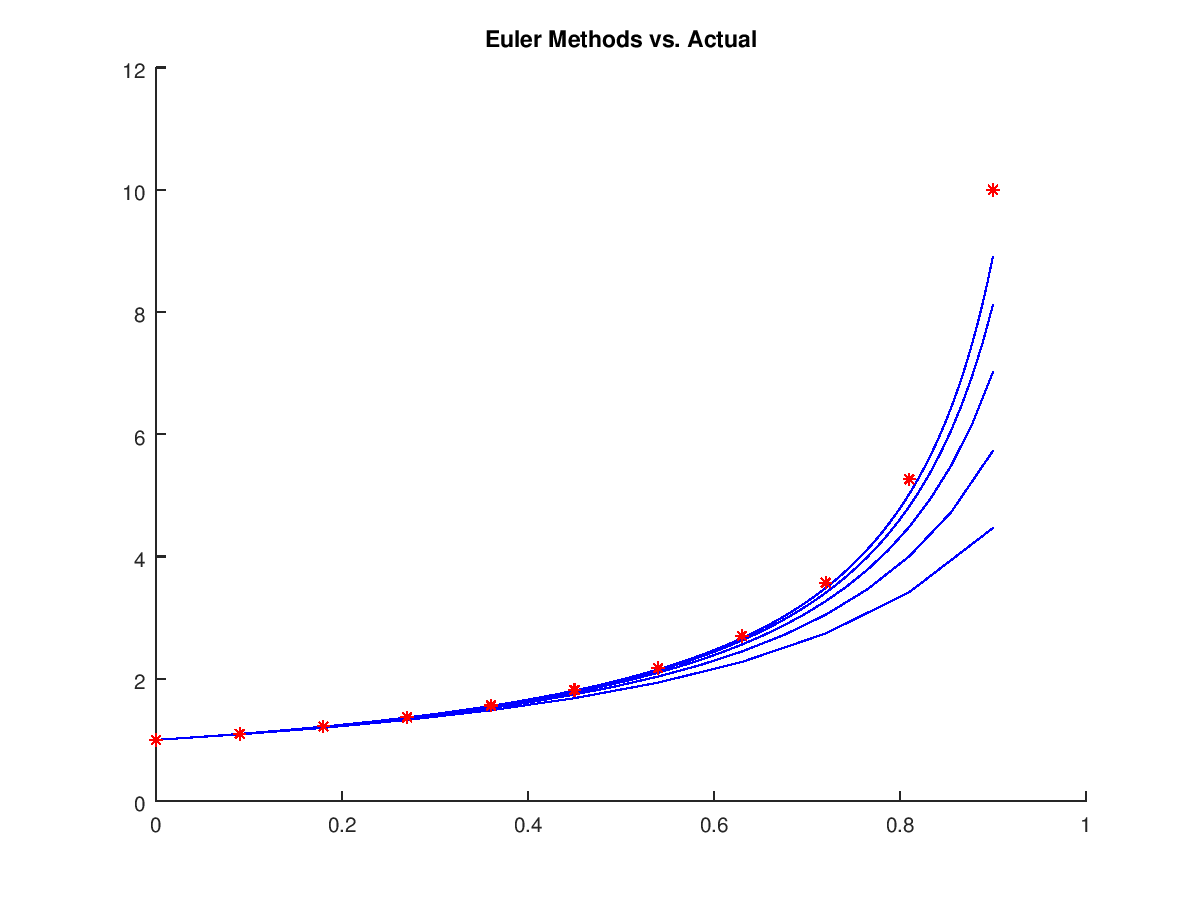
\includegraphics[height=6cm]{problem2_f}\\
Figure: Shown in blue is the approximate solution to the differential equation $y' = y^2$ using Euler estimations method with different $n's$ of 10, 20, 40, 80, and 160. Shown in red is the actual solution for the equation.

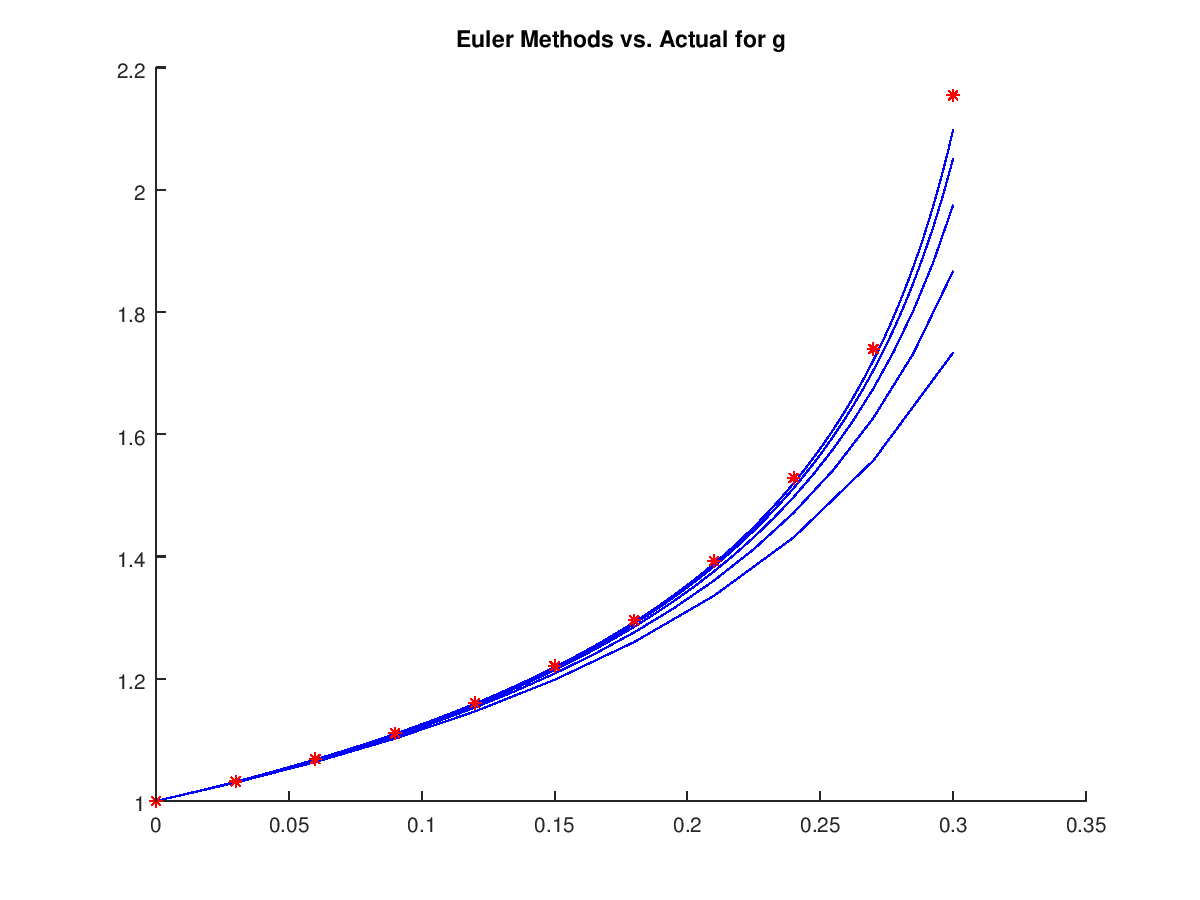
\includegraphics[height=6cm]{problem2_g}\\
Figure: Shown in blue is the approximate solution to the differential equation $y' = y^4$ using Euler method with different $n's$ of 10, 20, 40, 80, and 160. Shown in red is the actual solution for the equation.


\section{Newtons Method}
Newtons method uses the equation of the tangent line to find when a given equation equals zero. Below is the tangent line which is the starting point for the derivation of this method. 

	$ y = f'(x_n)(x - x_n) + f(x_n)$

If we then set $y$ equal to zero and solving for the next value of $x$ we are able to obtain the following equation which is then iterated on until a stoping criteria is met to find zeros.

	$ x_{n+1} = x_n - f(x_n) / f'(x_n) $

To implement this method we used two different approaches, the first is a sequential approach where a while loop is used to recalculate $x_{n+1}$ until the stop criteria is met, the second approach uses a recursive function to calculate and re-calculate $x_{n+1}$ until a base-case (stopping criteria) is met. Though the recursive solution is more elegant it does have some serious draw backs. One of these draw backs is when the tolerance variable is extremely low it will hit maximum recursive depth meaning the program has run out of memory. Even with this limitation the two implementations do return the same results. 

The following are the results after running the script with both approaches and with both initial guesses. 

\begin{lstlisting}
--- Project0 Netwon Methods ---
 Where, 
 f(x) = x^2 ,  g(x) = x^4
 f - g = x^2 - x^4
 fp = 2x - 4x^3
 Tollerance thershold = 1e-10
-- Guess 1 Method 1 (Sequential) --
 x0 = 2
chi=0.42857 xn = 1.5714
chi=0.29312 xn = 1.2783
chi=0.17868 xn = 1.0996
chi=0.081089 xn = 1.0185
chi=0.017733 xn = 1.0008
chi=0.00080692 xn = 1
chi=1.6299e-06 xn = 1
chi=6.6414e-12 xn = 1
 Result = 1
-- Guess 2 Method 1 (Sequential) --
 x0 = 1/4
chi=0.13393 xn = 0.11607
chi=0.058839 xn = 0.057232
chi=0.02871 xn = 0.028522
chi=0.014272 xn = 0.014249
chi=0.0071261 xn = 0.0071232
chi=0.0035618 xn = 0.0035614
chi=0.0017807 xn = 0.0017807
chi=0.00089034 xn = 0.00089034
chi=0.00044517 xn = 0.00044517
chi=0.00022258 xn = 0.00022258
chi=0.00011129 xn = 0.00011129
chi=5.5646e-05 xn = 5.5646e-05
chi=2.7823e-05 xn = 2.7823e-05
chi=1.3912e-05 xn = 1.3912e-05
chi=6.9558e-06 xn = 6.9558e-06
chi=3.4779e-06 xn = 3.4779e-06
chi=1.7389e-06 xn = 1.7389e-06
chi=8.6947e-07 xn = 8.6947e-07
chi=4.3473e-07 xn = 4.3473e-07
chi=2.1737e-07 xn = 2.1737e-07
chi=1.0868e-07 xn = 1.0868e-07
chi=5.4342e-08 xn = 5.4342e-08
chi=2.7171e-08 xn = 2.7171e-08
chi=1.3585e-08 xn = 1.3585e-08
chi=6.7927e-09 xn = 6.7927e-09
chi=3.3964e-09 xn = 3.3964e-09
chi=1.6982e-09 xn = 1.6982e-09
chi=8.4909e-10 xn = 8.4909e-10
chi=4.2455e-10 xn = 4.2455e-10
chi=2.1227e-10 xn = 2.1227e-10
chi=1.0614e-10 xn = 1.0614e-10
chi=5.3068e-11 xn = 5.3068e-11
 Result = 5.3068e-11
-- Guess 1 Method 2 (Recurive) --
 x0 = 2
chi=0.42857 xn = 1.5714
chi=0.29312 xn = 1.2783
chi=0.17868 xn = 1.0996
chi=0.081089 xn = 1.0185
chi=0.017733 xn = 1.0008
chi=0.00080692 xn = 1
chi=1.6299e-06 xn = 1
chi=6.6414e-12 xn = 1
 Result = 1
-- Guess 2 Method 1 (Recurive) --
 x0 = 1/4
chi=0.13393 xn = 0.11607
chi=0.058839 xn = 0.057232
chi=0.02871 xn = 0.028522
chi=0.014272 xn = 0.014249
chi=0.0071261 xn = 0.0071232
chi=0.0035618 xn = 0.0035614
chi=0.0017807 xn = 0.0017807
chi=0.00089034 xn = 0.00089034
chi=0.00044517 xn = 0.00044517
chi=0.00022258 xn = 0.00022258
chi=0.00011129 xn = 0.00011129
chi=5.5646e-05 xn = 5.5646e-05
chi=2.7823e-05 xn = 2.7823e-05
chi=1.3912e-05 xn = 1.3912e-05
chi=6.9558e-06 xn = 6.9558e-06
chi=3.4779e-06 xn = 3.4779e-06
chi=1.7389e-06 xn = 1.7389e-06
chi=8.6947e-07 xn = 8.6947e-07
chi=4.3473e-07 xn = 4.3473e-07
chi=2.1737e-07 xn = 2.1737e-07
chi=1.0868e-07 xn = 1.0868e-07
chi=5.4342e-08 xn = 5.4342e-08
chi=2.7171e-08 xn = 2.7171e-08
chi=1.3585e-08 xn = 1.3585e-08
chi=6.7927e-09 xn = 6.7927e-09
chi=3.3964e-09 xn = 3.3964e-09
chi=1.6982e-09 xn = 1.6982e-09
chi=8.4909e-10 xn = 8.4909e-10
chi=4.2455e-10 xn = 4.2455e-10
chi=2.1227e-10 xn = 2.1227e-10
chi=1.0614e-10 xn = 1.0614e-10
chi=5.3068e-11 xn = 5.3068e-11
 Result = 5.3068e-11
\end{lstlisting}

It is easy to see that in both approaches that $x_0 = 2$ converges quicker, however, it it finds the $1$ zeros while $x_0 = 1/4$ looks like it approaches $0$ the other zero. 

\section{First and Second Derivative}
The problem of finding the first and second derivative of an equation can be sometimes extremely hard by hand. For this problem it is possible to approximate the solution using matrix multiplication. This is accomplished by looking at the individual changes in $f(x)$ over time. This calculation can be accomplished by using a sparse matrix with -1 on the diagonal and 1 on the diagonal above that  and then multiple that matrix by values of the function. 

The following are the results of running this method on two functions $f(x) = x^2$ and $g(x) = x^4$. We this also compare the exact first and second derivatives to see how close the approximation is. 

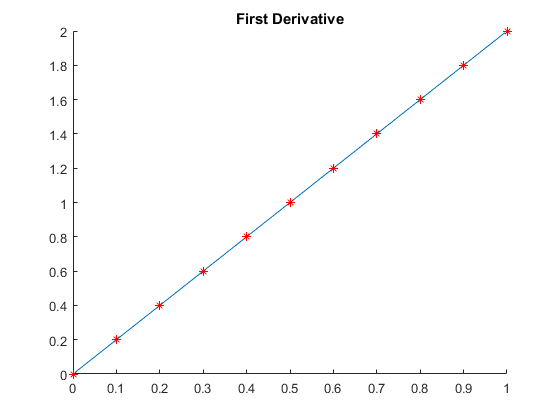
\includegraphics[height=6cm]{f_fp}\\
Figure : First derivative of $f$ is shown with the blue line is the approximation and the red line is the exact derivative. 

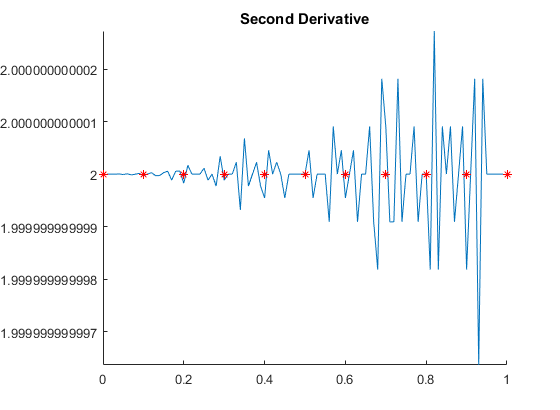
\includegraphics[height=6cm]{f_fpp}\\
Figure : Second derivative of $f$ is shown with the blue line is the approximation and the red line is the exact derivative. 

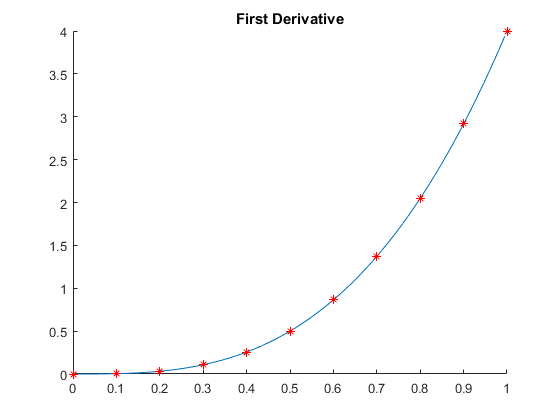
\includegraphics[height=6cm]{g_fp}\\
Figure : First derivative of $g$ is shown with the blue line is the approximation and the red line is the exact derivative. 

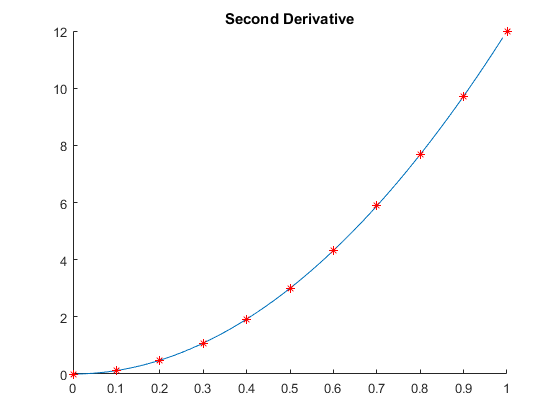
\includegraphics[height=6cm]{g_fpp}\\
Figure : Second derivative of $g$ is shown with the blue line is the approximation and the red line is the exact derivative. 


We can see from these figures that the approximation for the first and second derivative for both functions lay exactly on the actual derivative. 

\end{document}
